\documentclass[11pt]{article}
\usepackage[margin=1in]{geometry}
\usepackage{fontspec}
\usepackage{booktabs}
\usepackage{array}
\usepackage{tabularx}
\usepackage{threeparttable}
\usepackage{makecell}
\usepackage{float}
\usepackage{graphicx}
\usepackage{amsmath}
\usepackage{amssymb}
\usepackage[font=small,labelfont=bf]{caption}
\usepackage{natbib}
\usepackage{xurl}
\usepackage[hidelinks]{hyperref}
\usepackage{setspace}
\setstretch{1.15}
\graphicspath{{../figs/}}
\newcommand{\incAgree}{98.6}
\newcommand{\incRecall}{85}
\newcommand{\incPrecision}{91}
\newcommand{\nExanteLate}{244}
\newcommand{\nLeaderLate}{390}
\newcommand{\nTcpdCand}{570,241}
\newcommand{\mahaMargin}{1,217}
\newcommand{\mahaN}{7}
\newcommand{\mahaVotes}{62,934}
\newcommand{\nInd}{246,894}
\newcommand{\nIndContests}{41,495}
\newcommand{\nTreated}{3,144}
\newcommand{\nTreatedAll}{3,277}
\newcommand{\nTreatedTopTwo}{17}
\newcommand{\medIndShare}{0.33}
\newcommand{\medNamesakeVotes}{462}
\newcommand{\lsLeaderExact}{7.6}
\newcommand{\lsMinorExact}{2.9}
\newcommand{\lsLeaderRatio}{2.6}
\newcommand{\aeLeaderExact}{8.3}
\newcommand{\aeMinorExact}{4.8}
\newcommand{\aeLeaderRatio}{1.7}
\newcommand{\rkExact}{+7.7}
\newcommand{\rkExactSe}{1.4}
\newcommand{\rkInit}{+8.1}
\newcommand{\rkInitSe}{1.2}
\newcommand{\rkLook}{+4.6}
\newcommand{\rkLookSe}{0.9}
\newcommand{\rkPlExact}{+1.3}
\newcommand{\rkPlExactSe}{1.7}
\newcommand{\rkPlLook}{+2.3}
\newcommand{\rkPlLookSe}{0.9}
\newcommand{\lgExact}{+0.17}
\newcommand{\lgExactSe}{0.04}
\newcommand{\lgExactPct}{18}
\newcommand{\lgInit}{+0.16}
\newcommand{\lgInitSe}{0.03}
\newcommand{\lgInitPct}{18}
\newcommand{\lgPlExact}{-0.02}
\newcommand{\lgPlExactSe}{0.05}
\newcommand{\poExact}{-0.04}
\newcommand{\poExactSe}{0.12}
\newcommand{\poInit}{-0.11}
\newcommand{\poInitSe}{0.07}
\newcommand{\poLook}{-0.19}
\newcommand{\poLookSe}{0.06}
\newcommand{\divExact}{16}
\newcommand{\divInit}{15}
\newcommand{\tgWinRk}{+8.8}
\newcommand{\tgWinRkSe}{1.3}
\newcommand{\tgExRk}{+7.1}
\newcommand{\tgExRkSe}{1.1}
\newcommand{\tgAllRk}{+7.5}
\newcommand{\tgAllRkSe}{1.0}
\newcommand{\tgAllPo}{-0.37}
\newcommand{\tgAllPoSe}{0.09}
\newcommand{\tgLsLg}{+0.28}
\newcommand{\tgLsLgSe}{0.07}
\newcommand{\tgAeLg}{+0.14}
\newcommand{\tgAeLgSe}{0.03}
\newcommand{\phRkPost}{-3.7}
\newcommand{\phRkPostSe}{2.0}
\newcommand{\phRkTrendPost}{-4.3}
\newcommand{\phRkTrendPostSe}{3.0}
\newcommand{\phLgPost}{-0.11}
\newcommand{\phLgPostSe}{0.05}
\newcommand{\phLgTrendPost}{-0.09}
\newcommand{\phLgTrendPostSe}{0.08}
\newcommand{\phLgWin}{-0.11}
\newcommand{\phLgWinSe}{0.07}
\newcommand{\brRealT}{-2.3}
\newcommand{\brFakeMinT}{-2.8}
\newcommand{\brFakeMinYear}{1998}
\newcommand{\brFakeSig}{3}
\newcommand{\brFakeN}{15}
\newcommand{\esLate}{+0.26}
\newcommand{\esPost}{+0.08}
\newcommand{\esEarly}{+0.07}
\newcommand{\esMid}{+0.11}
\newcommand{\esFirst}{+0.28}
\newcommand{\esNineties}{+0.29}
\newcommand{\esLast}{+0.11}
\newcommand{\nMarginContests}{57,165}
\newcommand{\ovExactHas}{316}
\newcommand{\ovExactBound}{15}
\newcommand{\ovExactPoint}{1}
\newcommand{\ovExactLow}{0}
\newcommand{\ovExactHigh}{4}
\newcommand{\ovLookHas}{1,365}
\newcommand{\ovLookBound}{76}
\newcommand{\ovLookPoint}{12}
\newcommand{\ovLookLow}{4}
\newcommand{\ovLookHigh}{17}
\newcommand{\ovLookPointPct}{0.02}
\newcommand{\thirdOver}{45}
\newcommand{\nBiharCand}{646,399}
\newcommand{\nBiharContests}{155,194}
\newcommand{\bhRk}{-0.5}
\newcommand{\bhRkSe}{0.9}
\newcommand{\bhLg}{-0.01}
\newcommand{\bhLgSe}{0.02}
\newcommand{\bhPo}{-0.02}
\newcommand{\bhPoSe}{0.03}


\title{Do Namesakes Confuse Voters? Evidence from Six Decades of Indian Elections}
\author{Gaurav Sood\thanks{I thank Priyadarshi Amar for obtaining the Election Commission's statistical reports for the 2023--2026 assembly elections.}}
\date{\today}

\begin{document}
\maketitle

\begin{abstract}
\noindent Indian ballots often list minor independents who share a name with a leading candidate, and parties are widely reported to plant them to siphon votes. We ask three questions: do voters confuse namesakes with the candidates they resemble, how many votes does the confusion move, and is it enough to change who wins? Using \nTcpdCand{} Lok Sabha and assembly candidate records (1962--2026), we compare independents whose names resemble a leading party candidate with other independents in the same contest. Namesakes of leaders place \rkExact{} percentile points higher (SE \rkExactSe) among the contest's independents and poll about \lgExactPct\% more votes than a typical rival independent, while independents who resemble a minor party candidate gain nothing detectable. The gain is small in votes: the median namesake polls \medNamesakeVotes{} votes, and their mean vote count is no higher than other independents'. Counting every vote a runner-up's namesakes received, they exceeded the winning margin in \ovLookBound{} of \nMarginContests{} contests; counting only the votes attributable to the name, \ovLookPoint{} (95\% range \ovLookLow--\ovLookHigh). The 2015 rule adding candidate photographs to voting machines coincides with a smaller premium, but placebo break dates and a trend in the premium produce changes of the same size, so the data cannot attribute the decline to photographs. Bihar's panchayat elections show no namesake premium.
\end{abstract}

\section{Introduction}

Parties and campaign operatives in India are widely reported to recruit ``dummy'' candidates: citizens who share the name of a leading contender and file as independents, in the hope that some of the contender's voters mark the wrong line \citep{factly2019, diplomat2020}. The Election Commission of India cited the practice when it required electronic voting machines (EVMs) and ballot papers to carry candidate photographs from 1 May 2015 \citep{businessstandard2015}. Individual races look dramatic. In Mahasamund (Lok Sabha, 2014), Chandu Lal Sahu of the BJP won by \mahaMargin{} votes while \mahaN{} independents with the same or a same-sounding name polled \mahaVotes{} votes between them. The pattern is not chance: in Lok Sabha contests, a pair of one leading (top-two) candidate and one minor candidate is \lsLeaderRatio{} times as likely to share an exact name as a pair of two minor candidates (\lsLeaderExact{} versus \lsMinorExact{} per 10,000 pairs; in assemblies \aeLeaderRatio{} times, \aeLeaderExact{} versus \aeMinorExact{}).

Planting namesakes only matters politically if voters are fooled, and if enough are fooled to change results. Mahasamund illustrates the difficulty: the namesakes polled a lot, yet the candidate they resembled still won, and some of those votes would have gone to minor candidates anyway. This paper separates three questions. First, are voters confused, that is, does resembling a leader earn an independent votes it would not otherwise get? Second, how many votes does that move? Third, is it enough to overturn results? We then ask whether the 2015 photograph rule reduced confusion, and find that the data cannot answer that question.

\section{Data and Design}

\paragraph{Data.} We use every general-election candidate in the Trivedi Centre for Political Data's Lok Dhaba files \citep{agarwal2021}, which end with the 2019 Lok Sabha and the 2023 assembly elections, extended with the Election Commission's results for the 2024 Lok Sabha and the assemblies from November 2023 to 2026, which we put into TCPD's column layout with TCPD's own rules for its derived columns (\url{https://github.com/in-rolls/eci_results}; all are from the Commission's official statistical reports): \nTcpdCand{} candidate records after dropping by-elections and state-years whose names are printed mostly as initials. Names are compared at three levels: exact or spelling-equivalent (identical after folding spellings of one spoken name), differing only in initials (\emph{K.N. Rao} and \emph{Rao}), and look-alike (one name contains the other, or the given names are at least 0.7 similar after shared words are set aside). The first two together are \emph{close names}.

\paragraph{Comparison.} Planted namesakes are independents, and almost all of them poll little. Comparing them with every losing candidate would set them against runners-up who poll 30--40\% of the vote, so we compare independents with independents in the same contest. The sample is the \nInd{} independents placed third or lower in \nIndContests{} contests with at least two such independents; \nTreatedTopTwo{} of the \nTreatedAll{} independents who resemble a leader finished first or second, so this restriction drops almost no namesakes while removing strong rebel independents from the comparison group. Table~\ref{tab:targets} column 4 keeps all independents. An independent is treated if its name resembles a party candidate who finished first or second (the \emph{leader}). Because finishing first or second is itself an outcome, we also define the target before the election, as an incumbent or a national-party candidate (Table~\ref{tab:targets} column 3). TCPD identifies incumbents by linking candidates across elections, which the post-2023 results lack, so for every year we flag as incumbent the one candidate in each contest whose name best matches the winner of the seat's previous general election (token-set similarity of at least 90, seat boundaries unchanged, ties going to the winner's party). On TCPD's 2014--2023 rows this agrees with TCPD's flag for \incAgree\% of candidates; it finds \incRecall\% of TCPD's incumbents, and \incPrecision\% of those it flags are incumbents by TCPD's flag. National parties are TCPD's through 2023 and, from 2024, the six recognized by the Election Commission in April 2023 (BJP, INC, BSP, CPI(M), AAP, NPP). This gives \nExanteLate{} pre-defined namesakes in 2024--2026, against \nLeaderLate{} namesakes of leaders.

\paragraph{Outcomes.} Each answers a different question. The candidate's \emph{rank} among the contest's independents, scaled so the average independent sits at the 50th percentile, asks whether the name helps at all and ignores how large any vote total is. $\log(1+\text{votes})$ measures the proportional gain of a typical namesake. Votes estimated by Poisson regression measure the proportional gain in \emph{mean} votes; the mean is dominated by the few independents who poll thousands, so this is the outcome that most depends on who else is in the comparison group.

\paragraph{Estimator.} For independent $i$ in contest $c$,
\begin{equation}
Y_{ic} = \alpha_c + \sum_{k} \beta_{k} D_{ic}^{(k)} + \sum_{k} \delta_{k} P_{ic}^{(k)} + \gamma \log(1 + \text{Freq}_{i}) + \varepsilon_{ic},
\end{equation}
where $\alpha_c$ is a contest fixed effect, so every comparison is between independents on the same ballot. $D^{(k)}_{ic}$ marks resemblance to a leader at level $k$, and $P^{(k)}_{ic}$ marks resemblance to a party candidate who finished third or lower. That second set is a placebo: such a candidate's voters are too few for confusion to pay, but the candidate's name is drawn from the same local pool of common names, so if common names attract votes on their own, $\delta_k$ will pick it up. $\text{Freq}_i$ is how often the candidate's spelling appears among all candidates. Standard errors are clustered by constituency, because a constituency hosts many contests over six decades. Estimates come from \texttt{pyfixest}.

\section{Are Voters Confused?}

Table~\ref{tab:confusion} gives the answer. Independents whose names match a leader's exactly or by spelling place \rkExact{} percentile points (SE \rkExactSe) above the average independent on their ballot, and those differing only in initials \rkInit{} points (SE \rkInitSe). In log votes, an exact namesake polls \lgExact{} (SE \lgExactSe), about \lgExactPct\% more than a typical rival independent. The placebo shows that a common name alone does not do this: an independent who exactly matches a minor party candidate places \rkPlExact{} points higher (SE \rkPlExactSe) and polls \lgPlExact{} log points (SE \lgPlExactSe). Look-alikes are different. Their premium of \rkLook{} points (SE \rkLookSe) is about twice the placebo's \rkPlLook{} (SE \rkPlLookSe), so roughly half of the look-alike premium could be name commonness rather than confusion.

\begin{table}[htbp]
\centering\small
\caption{Do independents who resemble a leader poll more than other independents on the same ballot?}
\label{tab:confusion}
\begin{threeparttable}
\begingroup
\renewcommand\cellalign{t}
\renewcommand\arraystretch{1}
\setlength{\tabcolsep}{3pt}
\begin{tabularx}{\linewidth}{@{}>{\raggedright\arraybackslash}l>{\centering\arraybackslash}X>{\centering\arraybackslash}X>{\centering\arraybackslash}X}
\toprule
 & \multicolumn{1}{c}{Rank (percentile pts.)} & \multicolumn{1}{c}{Log(1 + votes)} & \multicolumn{1}{c}{Votes (Poisson)} \\
\cmidrule(lr){2-2} \cmidrule(lr){3-3} \cmidrule(lr){4-4}
 & (1) & (2) & (3) \\
\midrule
\addlinespace[1ex]
Exact / spelling & \makecell{7.73 \\ (1.44)} & \makecell{0.17 \\ (0.04)} & \makecell{-0.04 \\ (0.12)} \\
\addlinespace[0.5ex]
\addlinespace[0.5ex]
Initials differ & \makecell{8.06 \\ (1.24)} & \makecell{0.16 \\ (0.03)} & \makecell{-0.11 \\ (0.07)} \\
\addlinespace[0.5ex]
\addlinespace[0.5ex]
Look-alike & \makecell{4.62 \\ (0.94)} & \makecell{0.08 \\ (0.03)} & \makecell{-0.19 \\ (0.06)} \\
\addlinespace[0.5ex]
\addlinespace[0.5ex]
Placebo: exact / spelling & \makecell{1.26 \\ (1.68)} & \makecell{-0.02 \\ (0.05)} & \makecell{-0.02 \\ (0.15)} \\
\addlinespace[0.5ex]
\addlinespace[0.5ex]
Placebo: initials differ & \makecell{1.25 \\ (1.95)} & \makecell{0.03 \\ (0.05)} & \makecell{-0.02 \\ (0.16)} \\
\addlinespace[0.5ex]
\addlinespace[0.5ex]
Placebo: look-alike & \makecell{2.30 \\ (0.87)} & \makecell{0.07 \\ (0.03)} & \makecell{0.05 \\ (0.07)} \\
\addlinespace[0.5ex]
\addlinespace[0.5ex]
Log name frequency & \makecell{-0.19 \\ (0.06)} & \makecell{-0.01 \\ (0.00)} & \makecell{-0.01 \\ (0.00)} \\
\addlinespace[0.5ex]
\midrule
\addlinespace[1ex]
Contest fixed effects & x & x & x \\
\addlinespace[0.5ex]
\midrule
\addlinespace[1ex]
Independent namesakes of a leader & 3,144 & 3,144 & 3,144 \\
\addlinespace[0.5ex]
\addlinespace[0.5ex]
Contests & 41,495 & 41,495 & 41,495 \\
\addlinespace[0.5ex]
\addlinespace[0.5ex]
Candidates & 246,894 & 246,894 & 246,894 \\
\addlinespace[0.5ex]
\bottomrule
\end{tabularx}
\endgroup
\noindent\begin{minipage}{\linewidth}\smallskip\footnotesize
Independents placed third or lower, in contests with at least two of them. Rows 1-3: resemblance to a party candidate placed first or second; rows 4-6: to a party candidate placed third or lower. Standard errors clustered by constituency in parentheses.\end{minipage}

\end{threeparttable}
\end{table}

The premium does not depend on how the target is defined (Table~\ref{tab:targets}). The close-name rank premium is \tgWinRk{} (SE \tgWinRkSe) for namesakes of the winner and \tgExRk{} (SE \tgExRkSe) for namesakes of incumbents and national-party candidates, defined before the vote. It is larger in Lok Sabha contests (\tgLsLg{} log points, SE \tgLsLgSe) than in assembly contests (\tgAeLg, SE \tgAeLgSe), consistent with voters knowing less about candidates in constituencies of two million people.

\begin{table}[htbp]
\centering\small
\caption{The namesake premium across targets and samples.}
\label{tab:targets}
\textbf{A. Rank among the contest's independents (percentile points)}\par\smallskip
\begin{threeparttable}
\begingroup
\renewcommand\cellalign{t}
\renewcommand\arraystretch{1}
\setlength{\tabcolsep}{3pt}
\begin{tabularx}{\linewidth}{@{}>{\raggedright\arraybackslash}l>{\centering\arraybackslash}X>{\centering\arraybackslash}X>{\centering\arraybackslash}X>{\centering\arraybackslash}X>{\centering\arraybackslash}X>{\centering\arraybackslash}X}
\toprule
 & \multicolumn{1}{c}{Top-2 leader} & \multicolumn{1}{c}{Winner} & \multicolumn{1}{c}{Incumbent or national party} & \multicolumn{1}{c}{All independents} & \multicolumn{1}{c}{Lok Sabha} & \multicolumn{1}{c}{Assembly} \\
\cmidrule(lr){2-2} \cmidrule(lr){3-3} \cmidrule(lr){4-4} \cmidrule(lr){5-5} \cmidrule(lr){6-6} \cmidrule(lr){7-7}
 & (1) & (2) & (3) & (4) & (5) & (6) \\
\midrule
\addlinespace[1ex]
Close name & \makecell{7.91 \\ (0.96)} & \makecell{8.82 \\ (1.35)} & \makecell{7.09 \\ (1.13)} & \makecell{7.50 \\ (0.96)} & \makecell{11.26 \\ (2.54)} & \makecell{7.11 \\ (1.03)} \\
\addlinespace[0.5ex]
\addlinespace[0.5ex]
Look-alike & \makecell{4.64 \\ (0.95)} & \makecell{4.26 \\ (1.21)} & \makecell{3.93 \\ (0.94)} & \makecell{4.40 \\ (0.94)} & \makecell{9.17 \\ (2.03)} & \makecell{3.45 \\ (1.06)} \\
\addlinespace[0.5ex]
\midrule
\addlinespace[1ex]
Candidates & 246,894 & 246,894 & 246,894 & 254,991 & 48,728 & 198,166 \\
\addlinespace[0.5ex]
\bottomrule
\end{tabularx}
\endgroup
\noindent\begin{minipage}{\linewidth}\smallskip\footnotesize
 \end{minipage}

\end{threeparttable}\par\medskip
\textbf{B. Log(1 + votes)}\par\smallskip
\begin{threeparttable}
\begingroup
\renewcommand\cellalign{t}
\renewcommand\arraystretch{1}
\setlength{\tabcolsep}{3pt}
\begin{tabularx}{\linewidth}{@{}>{\raggedright\arraybackslash}l>{\centering\arraybackslash}X>{\centering\arraybackslash}X>{\centering\arraybackslash}X>{\centering\arraybackslash}X>{\centering\arraybackslash}X>{\centering\arraybackslash}X}
\toprule
 & \multicolumn{1}{c}{Top-2 leader} & \multicolumn{1}{c}{Winner} & \multicolumn{1}{c}{Incumbent or national party} & \multicolumn{1}{c}{All independents} & \multicolumn{1}{c}{Lok Sabha} & \multicolumn{1}{c}{Assembly} \\
\cmidrule(lr){2-2} \cmidrule(lr){3-3} \cmidrule(lr){4-4} \cmidrule(lr){5-5} \cmidrule(lr){6-6} \cmidrule(lr){7-7}
 & (1) & (2) & (3) & (4) & (5) & (6) \\
\midrule
\addlinespace[1ex]
Close name & \makecell{0.17 \\ (0.03)} & \makecell{0.17 \\ (0.03)} & \makecell{0.14 \\ (0.03)} & \makecell{0.13 \\ (0.03)} & \makecell{0.28 \\ (0.07)} & \makecell{0.14 \\ (0.03)} \\
\addlinespace[0.5ex]
\addlinespace[0.5ex]
Look-alike & \makecell{0.09 \\ (0.03)} & \makecell{0.06 \\ (0.03)} & \makecell{0.08 \\ (0.03)} & \makecell{0.07 \\ (0.03)} & \makecell{0.23 \\ (0.06)} & \makecell{0.05 \\ (0.03)} \\
\addlinespace[0.5ex]
\midrule
\addlinespace[1ex]
Candidates & 246,894 & 246,894 & 246,894 & 254,991 & 48,728 & 198,166 \\
\addlinespace[0.5ex]
\bottomrule
\end{tabularx}
\endgroup
\noindent\begin{minipage}{\linewidth}\smallskip\footnotesize
 \end{minipage}

\end{threeparttable}\par\medskip
\textbf{C. Votes (Poisson)}\par\smallskip
\begin{threeparttable}
\begingroup
\renewcommand\cellalign{t}
\renewcommand\arraystretch{1}
\setlength{\tabcolsep}{3pt}
\begin{tabularx}{\linewidth}{@{}>{\raggedright\arraybackslash}l>{\centering\arraybackslash}X>{\centering\arraybackslash}X>{\centering\arraybackslash}X>{\centering\arraybackslash}X>{\centering\arraybackslash}X>{\centering\arraybackslash}X}
\toprule
 & \multicolumn{1}{c}{Top-2 leader} & \multicolumn{1}{c}{Winner} & \multicolumn{1}{c}{Incumbent or national party} & \multicolumn{1}{c}{All independents} & \multicolumn{1}{c}{Lok Sabha} & \multicolumn{1}{c}{Assembly} \\
\cmidrule(lr){2-2} \cmidrule(lr){3-3} \cmidrule(lr){4-4} \cmidrule(lr){5-5} \cmidrule(lr){6-6} \cmidrule(lr){7-7}
 & (1) & (2) & (3) & (4) & (5) & (6) \\
\midrule
\addlinespace[1ex]
Close name & \makecell{-0.07 \\ (0.07)} & \makecell{-0.11 \\ (0.08)} & \makecell{-0.09 \\ (0.07)} & \makecell{-0.37 \\ (0.09)} & \makecell{0.06 \\ (0.12)} & \makecell{-0.22 \\ (0.06)} \\
\addlinespace[0.5ex]
\addlinespace[0.5ex]
Look-alike & \makecell{-0.19 \\ (0.06)} & \makecell{-0.19 \\ (0.07)} & \makecell{-0.15 \\ (0.06)} & \makecell{-0.29 \\ (0.08)} & \makecell{0.00 \\ (0.08)} & \makecell{-0.36 \\ (0.08)} \\
\addlinespace[0.5ex]
\midrule
\addlinespace[1ex]
Candidates & 246,894 & 246,894 & 246,894 & 254,989 & 48,728 & 198,166 \\
\addlinespace[0.5ex]
\bottomrule
\end{tabularx}
\endgroup
\noindent\begin{minipage}{\linewidth}\smallskip\footnotesize
 \end{minipage}

\end{threeparttable}
\par\smallskip\footnotesize
\emph{Note}: Close name is exact, spelling or initials resemblance; models also include log name frequency and contest fixed effects. Columns 1--3 vary the target: party candidates placed first or second, the winner, or incumbents and national-party candidates. Column 4 adds independents placed first or second. Standard errors clustered by constituency.
\end{table}

\section{How Many Votes?}

Confusion is real but small in votes. The median leader namesake in our sample polls \medNamesakeVotes{} votes. If the name multiplies a namesake's votes by $e^{\beta}$, the share owed to the name is $1-e^{-\beta}$: \divExact\% for exact namesakes and \divInit\% for initials. For the median namesake that is a few dozen votes.

The Poisson estimates in the third column of Table~\ref{tab:confusion} put an upper limit on this. A namesake's \emph{mean} votes are no higher than other independents' (exact: \poExact, SE \poExactSe; initials: \poInit, SE \poInitSe), and when independents who finished first or second are included they are lower (\tgAllPo, SE \tgAllPoSe; Table~\ref{tab:targets}, column 4). Namesakes rise above the typical independent, but they do not join the few independents with a real following, who account for most independent votes. Read together, the outcomes say that resemblance shifts a namesake's vote count proportionally, from very little to a little more.

\section{Is It Enough to Overturn Elections?}

A runner-up's namesake can have cost the runner-up the seat only if the votes the name attracted exceed the winning margin. Table~\ref{tab:overturn} counts such contests three ways. As an accounting upper bound, which treats every vote cast for the namesake as a vote meant for the runner-up, the runner-up's independent look-alikes polled more than the margin in \ovLookBound{} of the \ovLookHas{} contests where the runner-up had one. That bound means little on its own: the third-placed candidate's votes exceed the margin in \thirdOver\% of all contests. Counting only the votes owed to the name, using each tier's log premium, the number falls to \ovLookPoint{} contests (95\% range \ovLookLow--\ovLookHigh), or \ovLookPointPct\% of the \nMarginContests{} contests with a party runner-up. For exact namesakes it is \ovExactPoint{} (range \ovExactLow--\ovExactHigh). The Poisson estimates imply fewer still.

Two assumptions make these counts generous. Every vote owed to the name is assumed to have been meant for the runner-up rather than for the winner, another minor candidate, or abstention. And the proportional premium estimated for the typical namesake is assumed to apply to large namesakes too. Winners' namesakes cannot have changed results, since the candidate they resembled won.

\begin{table}[htbp]
\centering\small
\caption{Contests in which a runner-up's independent namesakes polled more than the winning margin.}
\label{tab:overturn}
\begin{threeparttable}
\begingroup
\renewcommand\cellalign{t}
\renewcommand\arraystretch{1}
\setlength{\tabcolsep}{3pt}
\begin{tabularx}{\linewidth}{@{}>{\raggedright\arraybackslash}l>{\centering\arraybackslash}X>{\centering\arraybackslash}X>{\centering\arraybackslash}X>{\centering\arraybackslash}X}
\toprule
 & \multicolumn{1}{c}{} & \multicolumn{3}{c}{Namesake votes exceed the margin} \\
\cmidrule(lr){2-2} \cmidrule(lr){3-5}
 & Runner-up has one & All votes (bound) & Votes owed to name & 95\% range \\
\midrule
\addlinespace[1ex]
Exact / spelling & 316 & 15 & 1 & 0-4 \\
\addlinespace[0.5ex]
\addlinespace[0.5ex]
Close name (adds initials) & 690 & 34 & 5 & 1-9 \\
\addlinespace[0.5ex]
\addlinespace[0.5ex]
Any look-alike & 1,365 & 76 & 12 & 4-17 \\
\addlinespace[0.5ex]
\bottomrule
\end{tabularx}
\endgroup
\noindent\begin{minipage}{\linewidth}\smallskip\footnotesize
Counts of contests among 57,165 general-election contests with a party runner-up. Votes owed to the name: each runner-up namesake's votes times 1 - exp(-b), b its tier's log premium in Table 1 (95\% range from b's confidence interval).\end{minipage}

\end{threeparttable}
\end{table}

\section{Did Candidate Photographs Reduce Confusion?}

The photograph rule is a natural test of the confusion account: once voters can see faces, a shared name should matter less. Comparing the premium before and after May 2015, it fell by \phLgPost{} log points (SE \phLgPostSe; Table~\ref{tab:photo}, column 4) and \phRkPost{} rank points (SE \phRkPostSe). The data do not support attributing that decline to the photographs, for three reasons.

First, the premium was unstable long before 2015 (Figure~\ref{fig:photo}, top). In log votes it was \esFirst{} in 1962--89 and \esNineties{} in the 1990s, fell to \esEarly{} in 2000--04 and \esMid{} in 2005--09, and rose to \esLate{} in 2010--April 2015. The post-rule values, \esPost{} in May 2015--19 and \esLast{} in 2020--26, are no lower than 2000--09. Second, a break placed at other dates produces changes of the same size (Figure~\ref{fig:photo}, bottom). The real date gives $t=\brRealT$; a break in \brFakeMinYear{} gives $t=\brFakeMinT$, and \brFakeSig{} of \brFakeN{} placebo dates reach $|t|>1.96$. Third, allowing the premium to trend linearly leaves a change at May 2015 of \phLgTrendPost{} (SE \phLgTrendPostSe), and restricting to 2005--2019 gives \phLgWin{} (SE \phLgWinSe). Neither is distinguishable from zero.

Two more reasons for caution. The rule applied nationwide on one date, so the before-and-after comparison is one event, however many contests contribute to it. And the rule may have changed who runs as a namesake: if parties stopped planting them, the remaining namesakes are a different group.

\begin{table}[htbp]
\centering\small
\caption{The namesake premium before and after the May 2015 photograph rule.}
\label{tab:photo}
\begin{threeparttable}
\begingroup
\renewcommand\cellalign{t}
\renewcommand\arraystretch{1}
\setlength{\tabcolsep}{3pt}
\begin{tabularx}{\linewidth}{@{}>{\raggedright\arraybackslash}l>{\centering\arraybackslash}X>{\centering\arraybackslash}X>{\centering\arraybackslash}X>{\centering\arraybackslash}X>{\centering\arraybackslash}X>{\centering\arraybackslash}X}
\toprule
 & \multicolumn{3}{c}{Rank (percentile pts.)} & \multicolumn{3}{c}{Log(1 + votes)} \\
\cmidrule(lr){2-4} \cmidrule(lr){5-7}
 & \multicolumn{1}{c}{1962-2026} & \multicolumn{1}{c}{+ trend} & \multicolumn{1}{c}{2005-2019} & \multicolumn{1}{c}{1962-2026} & \multicolumn{1}{c}{+ trend} & \multicolumn{1}{c}{2005-2019} \\
\cmidrule(lr){2-2} \cmidrule(lr){3-3} \cmidrule(lr){4-4} \cmidrule(lr){5-5} \cmidrule(lr){6-6} \cmidrule(lr){7-7}
 & (1) & (2) & (3) & (4) & (5) & (6) \\
\midrule
\addlinespace[1ex]
Close name & \makecell{9.41 \\ (1.22)} & \makecell{9.82 \\ (2.06)} & \makecell{9.26 \\ (1.85)} & \makecell{0.21 \\ (0.03)} & \makecell{0.19 \\ (0.05)} & \makecell{0.19 \\ (0.05)} \\
\addlinespace[0.5ex]
\addlinespace[0.5ex]
Close name x after May 2015 & \makecell{-3.67 \\ (1.97)} & \makecell{-4.30 \\ (3.05)} & \makecell{-1.85 \\ (3.06)} & \makecell{-0.11 \\ (0.05)} & \makecell{-0.09 \\ (0.08)} & \makecell{-0.11 \\ (0.07)} \\
\addlinespace[0.5ex]
\addlinespace[0.5ex]
Close name x decades from May 2015 &  & \makecell{0.32 \\ (1.08)} &  &  & \makecell{-0.01 \\ (0.03)} &  \\
\addlinespace[0.5ex]
\addlinespace[0.5ex]
Look-alike & \makecell{5.32 \\ (1.10)} & \makecell{2.56 \\ (2.18)} & \makecell{1.88 \\ (2.06)} & \makecell{0.11 \\ (0.03)} & \makecell{0.03 \\ (0.06)} & \makecell{0.01 \\ (0.05)} \\
\addlinespace[0.5ex]
\addlinespace[0.5ex]
Look-alike x after May 2015 & \makecell{-2.38 \\ (2.06)} & \makecell{1.40 \\ (3.25)} & \makecell{-2.89 \\ (3.50)} & \makecell{-0.08 \\ (0.05)} & \makecell{0.03 \\ (0.09)} & \makecell{-0.06 \\ (0.09)} \\
\addlinespace[0.5ex]
\addlinespace[0.5ex]
Look-alike x decades from May 2015 &  & \makecell{-1.58 \\ (1.03)} &  &  & \makecell{-0.04 \\ (0.03)} &  \\
\addlinespace[0.5ex]
\midrule
\addlinespace[1ex]
Contest fixed effects & x & x & x & x & x & x \\
\addlinespace[0.5ex]
\midrule
\addlinespace[1ex]
Candidates & 246,894 & 246,894 & 57,629 & 246,894 & 246,894 & 57,629 \\
\addlinespace[0.5ex]
\bottomrule
\end{tabularx}
\endgroup
\noindent\begin{minipage}{\linewidth}\smallskip\footnotesize
Sample as in Table 1. Trend terms are in decades from 1 May 2015. Standard errors clustered by constituency in parentheses.\end{minipage}

\end{threeparttable}
\end{table}

\begin{figure}[htbp]
\centering
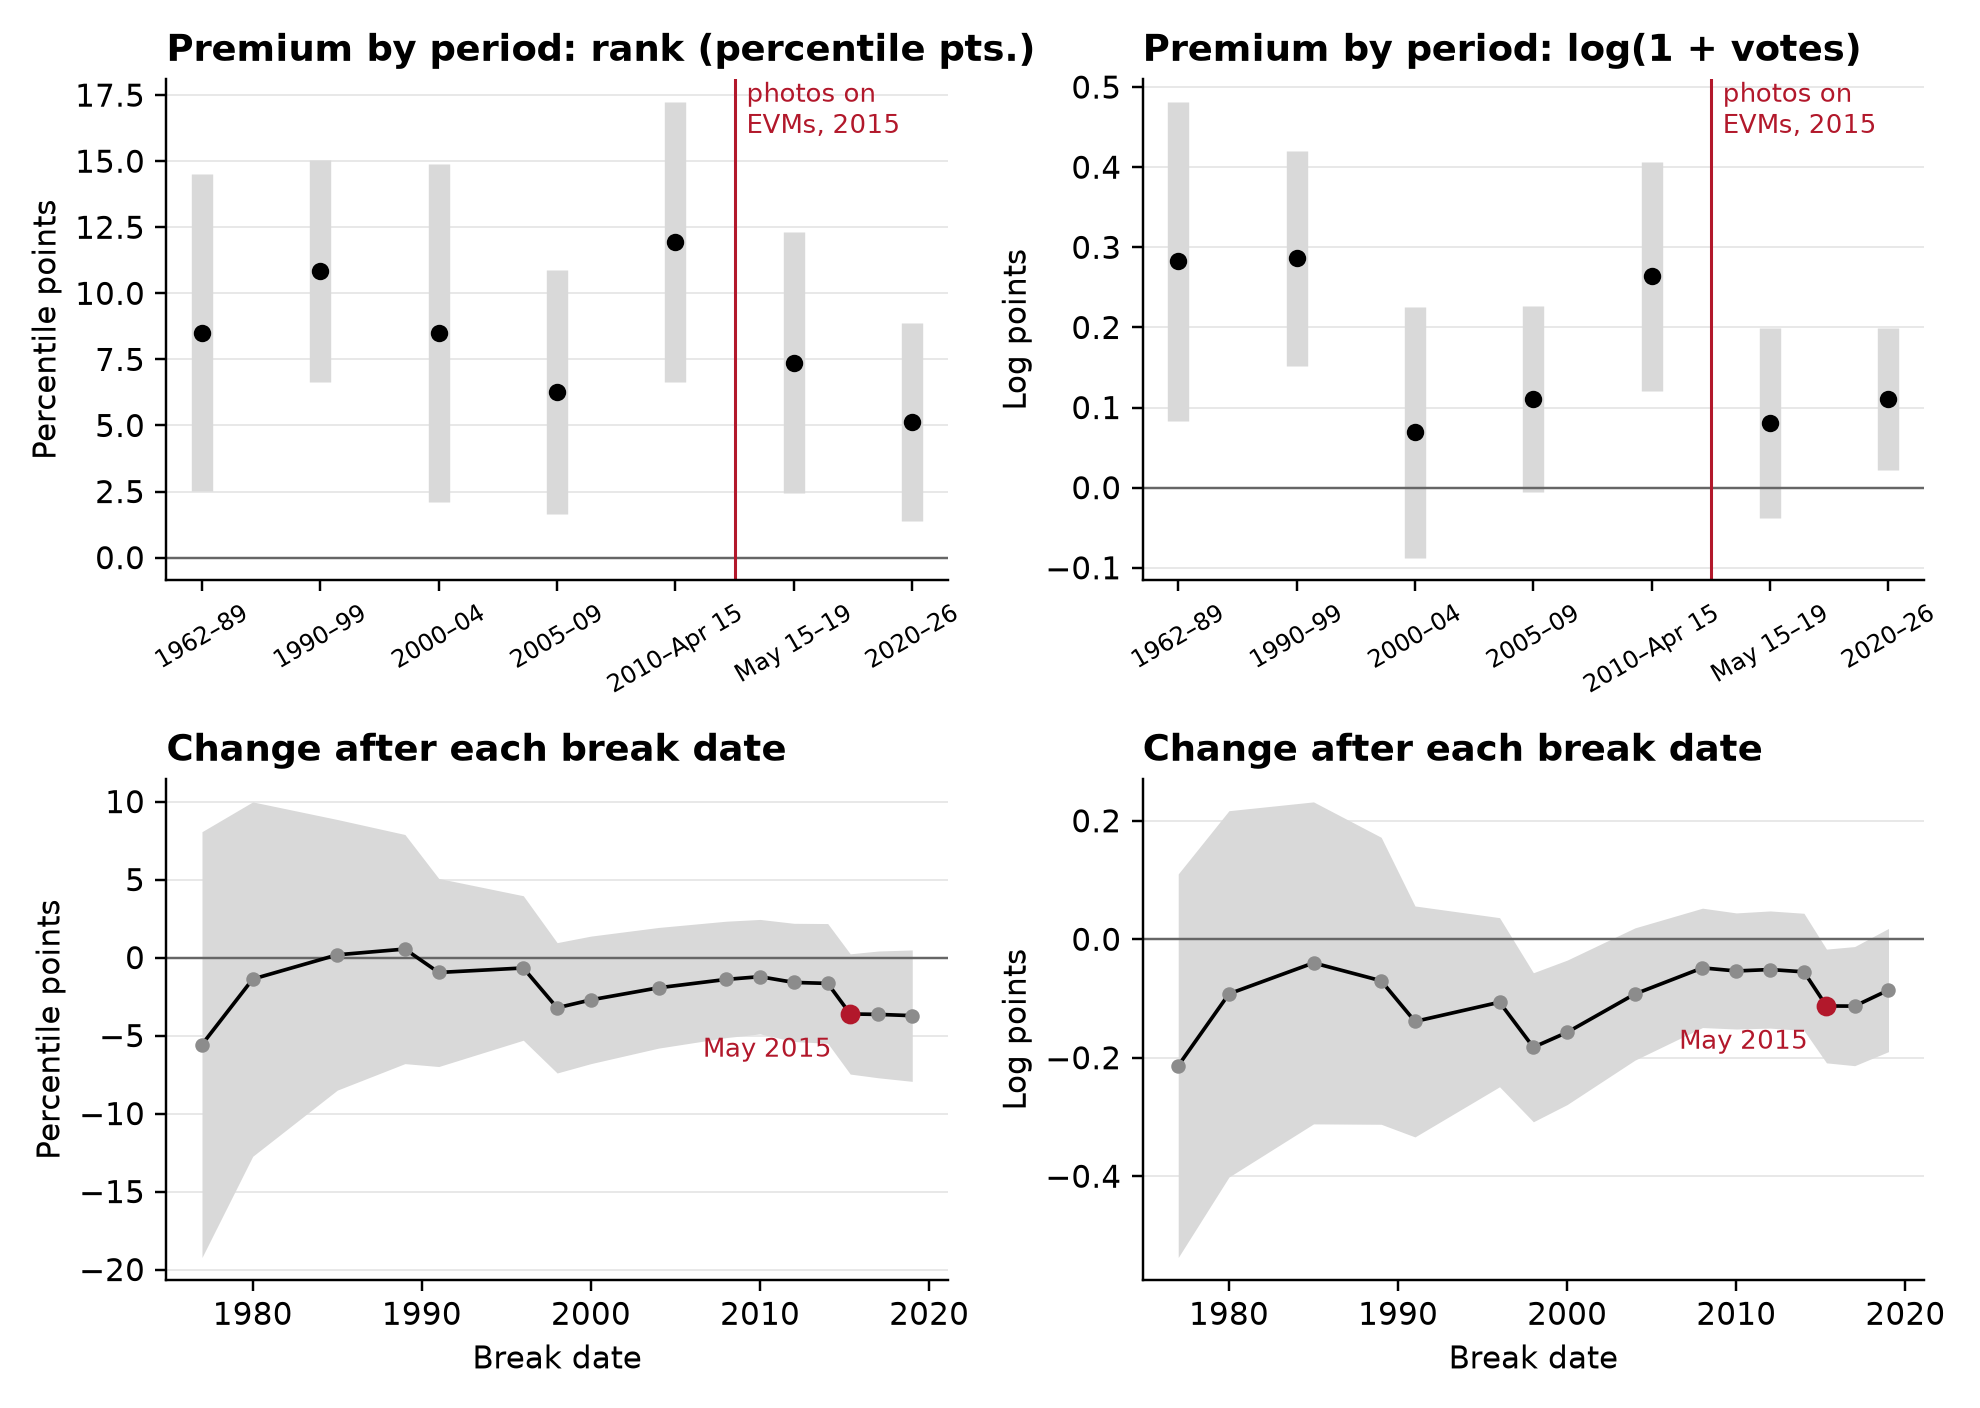
\includegraphics[width=\linewidth]{photo_rule.png}
\caption{Top: close-name premium by period; the red line marks 1 May 2015. Bottom: the estimated change in the premium after each candidate break date, from a model with one break (Table~\ref{tab:photo}, columns 1 and 4); gray dots are placebo dates and red marks the photograph rule. Gray bars and bands are 95\% confidence intervals. Standard errors clustered by constituency.}
\label{fig:photo}
\end{figure}

\section{Local Elections: Bihar's Panchayats}

Bihar's 2016 and 2021 panchayat elections cover \nBiharCand{} candidates placed third or lower in \nBiharContests{} contests across all six offices, from ward member to zila parishad. Candidates run without party labels, so the comparison is among all candidates placed third or lower. These elections are run by the State Election Commission, not the Election Commission of India, and we have not established whether their ballots carried photographs. Candidates who share the winner's name show no premium (Table~\ref{tab:bihar}): \bhRk{} rank points (SE \bhRkSe), \bhLg{} log points (SE \bhLgSe). In wards of a few hundred voters, who know the candidates personally, a shared name appears not to mislead.

\begin{table}[htbp]
\centering\small
\caption{Bihar panchayat elections (2016, 2021): candidates who resemble the winner, against others placed third or lower.}
\label{tab:bihar}
\begin{threeparttable}
\begingroup
\renewcommand\cellalign{t}
\renewcommand\arraystretch{1}
\setlength{\tabcolsep}{3pt}
\begin{tabularx}{\linewidth}{@{}>{\raggedright\arraybackslash}l>{\centering\arraybackslash}X>{\centering\arraybackslash}X>{\centering\arraybackslash}X}
\toprule
 & \multicolumn{1}{c}{Rank (percentile pts.)} & \multicolumn{1}{c}{Log(1 + votes)} & \multicolumn{1}{c}{Votes (Poisson)} \\
\cmidrule(lr){2-2} \cmidrule(lr){3-3} \cmidrule(lr){4-4}
 & (1) & (2) & (3) \\
\midrule
\addlinespace[1ex]
Same name / alias & \makecell{-0.47 \\ (0.88)} & \makecell{-0.01 \\ (0.02)} & \makecell{-0.02 \\ (0.03)} \\
\addlinespace[0.5ex]
\addlinespace[0.5ex]
One name contains the other & \makecell{-5.31 \\ (1.76)} & \makecell{-0.09 \\ (0.04)} & \makecell{-0.03 \\ (0.07)} \\
\addlinespace[0.5ex]
\addlinespace[0.5ex]
Similarity 0.8+ & \makecell{-0.91 \\ (1.50)} & \makecell{-0.01 \\ (0.03)} & \makecell{-0.03 \\ (0.05)} \\
\addlinespace[0.5ex]
\addlinespace[0.5ex]
Similarity 0.6-0.8 & \makecell{0.09 \\ (0.50)} & \makecell{-0.00 \\ (0.01)} & \makecell{-0.01 \\ (0.02)} \\
\addlinespace[0.5ex]
\midrule
\addlinespace[1ex]
Contest fixed effects & x & x & x \\
\addlinespace[0.5ex]
\midrule
\addlinespace[1ex]
Contests & 155,194 & 155,194 & 155,194 \\
\addlinespace[0.5ex]
\addlinespace[0.5ex]
Candidates & 646,399 & 646,399 & 646,399 \\
\addlinespace[0.5ex]
\bottomrule
\end{tabularx}
\endgroup
\noindent\begin{minipage}{\linewidth}\smallskip\footnotesize
Bihar panchayat candidates (2016, 2021, all six offices) placed third or lower, in contests with complete vote counts and at least two such candidates. Resemblance is to the contest's winner. All models control for log name frequency. Standard errors clustered by contest.\end{minipage}

\end{threeparttable}
\end{table}

\section{Conclusion}

Voters are confused by namesakes: independents who resemble a leading candidate consistently outpoll other independents on the same ballot, and independents who resemble a minor candidate do not. The confusion moves few votes. Namesakes rise from very few votes to slightly more, and even counting generously, the votes owed to a runner-up's namesakes exceeded the winning margin in about \ovLookPoint{} of \nMarginContests{} contests over six decades. Adding up every vote a namesake received, as press accounts do, gives \ovLookBound{} such contests instead of \ovLookPoint{}. Whether the 2015 photographs reduced confusion cannot be settled with these data, because the premium moved by as much at other dates.

\bibliographystyle{apsr}
\bibliography{references}

\end{document}
